% $Id: ESMF_archdoc.tex,v 1.2 2002/02/20 17:38:37 cdeluca Exp $

%
\documentclass[]{article}

\usepackage{epsf}
\usepackage{html}
\usepackage[T1]{fontenc}

\textwidth 6.5in
\textheight 8.5in
\addtolength{\oddsidemargin}{-.75in}

\begin{document}

\bodytext{BGCOLOR=white LINK=#083194 VLINK=#21004A}

\begin{titlepage}

\begin{center}
{\Large Earth System Modeling Framework } \\
\vspace{.25in}
{\Large {\bf ESMF Architecture}} \\
\vspace{.25in}
{\large {\it DRAFT}}
\vspace{.5in}
\end{center}

\begin{latexonly}
\vspace{5.5in}
\begin{tabular}{p{5in}p{.9in}}
\hrulefill \\
\noindent {\bf NASA High Performance Computing and Communications Program} \\
\noindent Earth and Space Sciences Project \\
\noindent CAN 00-OES-01 \\
\noindent http://www.esmf.ucar.edu \\
\end{tabular}
\end{latexonly}

\end{titlepage}

\tableofcontents

\newpage

%\section{Overview}

ESMF User's Guide
Quick start
Brief background
Design discussion
Overview of the directory structure / build system
Adopting the ESMF

ESMF Reference Manual
Public interfaces by class
Glossary

Design discussion

{\it 
In this section, we describe: 
\begin{itemize}
\item the goals and unique role of ESMF in Earth science;
\item the relevant features of the problem domain that ESMF encompasses; and
\item the key design features that are derived from the requirements of the ESMF domain and enable the ESMF to satisfy its goals. 
\end{itemize}
}

The {\bf Earth System Modeling Framework (ESMF)} is a software toolkit that increases software reuse, component interoperability, performance portability, and ease of use in Earth science applications.  The focus on Earth systems - a diverse but bounded domain - is critical to the ability of the ESMF to achieve its goals.  This is where the ESMF's value and capability come from - enabling interoperability but able to retain some efficiency and structure because the domain is bounded.  The scope is also unique - there are larger projects and smaller projects, but only ESMF spans institutions that are all interested in collaboration. The fifteen initial testbeds for the ESMF represent a wide range of research and operational applications in climate, weather, and data assimilation \cite{ref:models}.  Thus the ESMF must efficiently support a variety of grids, programming paradigms, and computing platforms.  However, the ESMF domain is restricted enough to allow the creation of specific data and control constructs.  A challenge of the project is to support high-performance operations in the face of the generality that's required.  Commonality in applications can be found at both the {\bf infrastructure} level, in model development tools for communication, I/O, time management, and other basic functions; and at the {\b superstructure} level, in an architecture and standards for combining geophysical components into applications.

The ESMF design is rooted in the requirements and characteristics of the applications that the framework must support.  In the sections below, these characteristics are described.  Then we describe the major architectural implications that spring from the nature of thhe domain

The key characteristics of the Earth science code that the ESMF must address are as follows.
\begin{enumerate}

\item Applications contain sets of complex software components that represent different 
physical domains, such as land, ocean, atmosphere and sea ice.  Other components may perform data assimilation 
or analysis.  These components are "coupled" so that the output fields of some of the components are used 
as the input fields for other components.  Coupling may include data transfers, unit conversions, flux 
calculations, regridding, data transfers, and other transformations.  The software that couples 
components is often viewed as a component itself.  

\item The same models or components may be run in a variety of configurations.  Scientists may swap in
alternative implementations of a domain or function in order to create new applications (e.g., different 
ocean models, different dynamical cores); may use different subsets and combinations of a particular set of 
components (e.g., an atmospheric model may be run with an ocean model for a hurricane application, and 
with a full complement of land, ocean, and sea ice models for a climate simulation); may run ensembles of the same component; and as a matter of course attempt endless variations and combinations of these research strategies.

\item Applications run on a variety of parallel computing systems and require high performances. 

\item Applications have many diverse users, from graduate students to software engineers to .  Applications are under continuous 
scientific development, and scientists and developers frequently wish to modify and update the code.

\end{enumerate}

The characteristics above inform a software architecture.  The key architectural features of ESMF are described below.

\begin{description}
\item[Component-based architecture]  Applications running under ESMF are organized as sets of interacting 
{\bf Components}.  A Component is
a software representation of some domain or function; for example, a land model or data assimilation 
system.  All Components share common behavior in ESMF.  This architectural model lends itself naturally to systems 

\item[Types of Components]  ESMF Components fall into a number of categories.  The two primary types are Gridded 
Components ({\tt ESMF\_GridComp}) and ESMF Coupler Components ({\tt ESMF\_CplComp}).  A Gridded Component represents 
a physical domain that contains fields discretized on a grid.  A Coupler Component 

\item[Local communication]

One of the important features of the ESMF architecture is that all communication between Gridded Components is 
local.  Another way of stating this is that all inter-component communication is mediated by a Coupler Component.    
\end{description}











%\section{Requirements}
%% $Id: ESMF_req.tex,v 1.2 2001/11/15 22:56:38 dneckels Exp $
\section{Requirements}

The Earth System Modeling Framework (ESMF) will consist of an interface
specification and a reference implementation.  The ESMF is intended to 
facilitate coupling of model components and to support lower-level
non-scientific tasks on high performance computer platforms.

The ESMF will support predictive models of the atmosphere, ocean, land and
sea ice and data assimilation systems.

More detailed functional requirements will be prepared as the project 
proceeds.

\subsection{Functional Requirements}

\subsubsection{Coupling Superstructure}

The ESMF will provide a coupling mechanism that performs regridding,
interpolation and communication of gridded, distributed data.  The 
data may represent multiple fields or a single field, may be in the
same or different executables, may be in code segments executing 
synchronously or asynchronously, and may be distributed among nodes
and/or partitioned among multiple threads.

\subsubsection{Parallel Support Layer}

The ESMF will provide the software necessary to support the data
decomposition and communication requirements of the individual components
and will do so in a way that is consistent with the superstructure.
This layer will include
tools for describing a wide variety of grids and decompositions,
and for performing high-level collective manipulations of fields defined
on those grids.  The software for specifying decompositions should support
default decompositions and dynamic load balancing.

\subsubsection{Utility Infrastructure}

The ESMF will include general purpose utility routines for use by both 
the coupling mechanism and application codes.  These include
performance profiling, time management and error handling.

The ESMF will support I/O of self-describing data in netCDF, HDF, 
binary, GRIB and BUFR data formmats.  Others such as the EOS HDF and ODF 
data formats are desired but not required.  The I/O utilities will 
have generic interfaces for ease of use, and will be high-performance.

\subsubsection{Evaluation Suite}

The ESMF will be distributed with a suite of representative components
that will demonstrate its usage.

\subsection{General Computational Requirements}

\subsubsection{Performance Portability}

Portability and computational efficiency over a wide range of platforms
is essential.  ESMF must be supported on the following platforms:
\begin{itemize}
\item Cray T3E (initial ESS testbed)
\item IBM SP
\item SGI Origin 2000
\item Compaq ES40
\item PC Linux platforms (including cluster)
\end{itemize}

Optimized performance on scalar architectures with moderate numbers of 
processors (100-1000) is the highest priority. 

Because many of the platforms listed above support multiple 
layers of parallelism (e.g. MPI, OpenMP),  the framework
must support message-based and thread-based parallelism and
hybrid combinations of the two approaches.

The framework will not increase the execution time of an existing code
written without the framework by more than 10\%.

The framework must include performance measurement tools. 

\subsubsection{Language}

ESMF utility and coupling software must have both Fortran 90 and
C/C++ bindings.

\subsubsection{Grids}

ESMF must support the coupling of components that are discretized on:
\begin{itemize}
\item logically rectangular grids
\item reduced (cut-out) and regional grids
\item unstructured grids (e.g., land grids, observations)
\item phase space grids (e.g., spectral, Fourier)
\item nested and adaptive grids
\item cubed sphere and icosahedral grids
\end{itemize}

In addition we require support for describing masked regions and
halo regions.

\subsubsection{Runtime Configurability}

ESMF must allow domain decomposition and the number of processors and/or
nodes to be configurable at runtime.  Other types of runtime configurability
may be permitted if acceptable performance is sustained.

\subsubsection{Fault Tolerance}

Error reporting must be handled consistently and with ample information
relayed to the user.  In situations where the components fail,
the ESMF will have a mechanism to detect the failure and shut down the
entire application.

\subsection{Design, Implementation and Maintenance Requirements}

\subsubsection{Flexibility and Extensibility}

Layers of the framework will be designed to survive restructuring of
other parts of the framework and user-supplied components.  For example,
the coupling layers should be able to adapt to different implementations
and data structures of component models.

\subsubsection{Ease of Adoption}

It must be straightforward to integrate ESMF into an application that
is reasonably modular.  We adopt as a goal that such applications should
need to modify no more than 2\% of their source code to utilize the coupling
features of ESMF.

\subsubsection{Ongoing Support}

The ESMF must be maintained as a long-term commitment by at least one
institution.  This maintenance must extend beyond adaptation to the 
computational environment, and must include an ongoing research component
dedicated to increasing the performance, flexibility and functionality of
the software.












%\section{Architecture}
%\input{ESMF_arch}

%\section{Scope}
\section{Scope of the ESMF}
\label{sec:shortscope}
The ESMF includes 1) services and standards for coupling high-level model components,
and 2) an infrastructure of general utilities for composing model components.  The model
components we will support initially are those included in the ESMF {\it Joint Milestone Codeset}, 
or JMC.  The JMC consists of climate, weather and data assimilation codes developed by 
ESMF investigators and their colleagues (see \htmladdnormallink
{http://www.esmf.ucar.edu/main\_site/resources}{http://www.esmf.ucar.edu/main\_site/resources}).  
These include regional and global atmospheres, regional and global oceans, land models, 
sea ice models, and data assimilation 
systems.  Each model component will need to recode or wrap its internal data structures in 
order to provide a standard ESMF interface and employ ESMF intercomponent communications.  
The ESMF coupling services will include software for representing data distributions, 
interpolating and redistributing gridded data, and load balancing computations.

Coupling services will be built upon a base of general data structures and utilities.  Supporting the coupling services and accessible to model developers are a set of 
general ESMF utilities.  These include error handling, timing and profiling, 
message logging, low-level I/O and communication, time management, and parameter 
specification.











%\section{Terminology}
\section{General Design Concepts}

Given the computational demands of Earth system modeling, the ESMF is by 
necessity complicated software running on complicated hardware.  However,
our goal is to develop a framework that is straightforward to understand and 
start using, reasonable to maintain, and amenable to extension.  To these 
ends we have adopted a design approach that modularizes the framework in a 
systematic and intuitive way.  Our architecture combines elements of 
object-oriented design, component-based design, and software layering, 
complementary approaches for ordering and decomposing software that apply
at different scales.  Object-oriented design organizes software into families 
of related structures that include even 
small data elements and minor functions.  Component-based design addresses 
larger software elements that are consistently defined and that interact
in a prescribed manner.  By layering we mean roughly apportioning elements 
of a software system into a few levels of a calling hierarchy.
All of these are useful conceptual tools for designing, understanding, and
explaining the structure of ESMF.

\subsection{Object-Oriented Design}

The ESMF is being designed using object-oriented (OO) principles.  OO design
is based on {\it classes}, which organize data, attributes, and associated 
operations into well-defined structures.  The OO approach distinguishes between 
the abstract concept of a class and an actual implementation or instance of the 
class, which is called an {\it object}.  The actual implementation of an 
abstract {\it operation} is called a {\it method}.

OO design is characterized by {\it encapsulation}, {\it inheritance}, and 
{\it polymorphism}.  Encapsulation means making data 
private to a particular class so that the underlying representation
can be changed or extended without changing the user interface to the class.
Inheritance allows specialized classes to inherit standard behavior from one
or more base
classes.  Polymorphism allows a single method to accept a variety of 
different argument lists when performing conceptually similar operations.  
Together these OO strategies help to organize and streamline codes, making 
them more flexible, maintainable, and extensible. 

In this document we use the Unified Modeling Language (UML) as a visual tool 
to express the structure of 
classes, to define the relationships between classes, and to describe sequences
of actions.  The diagrams are reasonably intuitive, and we provide 
only a basic explanation of concepts.  A reader interested in more detail should 
refer to a text such as ``The Unified Modeling Language Reference Manual.''

\subsection{Component-Based Design}

In this section we describe the features of component-based software 
architecture, then outline how the ESMF borrows from that model.  Unlike
OO design, the basic concepts of component-based design are not especially
easy to grasp and are not widely understood throughout the Earth system 
modeling community.  We therefore go into some detail.

In component-based design, applications are constructed using software entities 
called components, which are accessed only through {\it interfaces}.  
An interface is an array of function pointers.  Components usually have multiple 
interfaces, with each interface representing a collection of functionally 
related methods.  In addition to components, component 
architectures must define some sort of control mechanism that can handle tasks 
such as acquiring computing resources and starting an application, 
and creating, running, sequencing and synchronizing components.  We'll refer to
this mechanism as the Object Request Broker (ORB), as it's called in CORBA.  In the 
Common Component Architecture, this is called the framework - a different usage
of the word than we are accustomed to in ESMF.

The component model gets more complicated when, as in most ESMF applications, 
an application contains multiple processes.  Calling a 
method using a function pointer requires that the calling code share the 
same process as the called function.  

In COM and CORBA, component {\it proxies} are defined across
all the processes in the application.  A component proxy consists of gutted 
versions of all the functions in the interfaces of the component.  If the 
called function shares the same process as the caller, the proxy just 
calls the local function.  If the called component is in a different process, 
the proxy initiates some action such as a RPC through which a {\it stub} in 
the remote process actually makes the function call.\footnote{Different 
component systems call proxies and 
stubs by different names - skeletons, etc., but the concept remains the same.}  
The CCA architecture gets around this complication by 
requiring that all cross-process communication occur within a component, and
that all inter-component calls exchange only local data.  So, for example,
if you wanted to transfer data between two CCA components A and B, you would need 
to define a third component C on the union of A and B's processors and perform
the data transfer entirely within component C.

Another feature common to component architectures is an Interface Definition 
Language (IDL).  This is a language-independent way to express 
interfaces.  \footnote{In practice IDLs tend to look a lot like C++.}  Although 
an IDL isn't central to the notion of component architectures, it does enable 
niceties such as allowing the ORB to automatically generate proxies and stubs.

\subsection{Layered Architecture}

The ESMF and the applications that use it will be layered.  Layering generally 
refers to a calling hierarchy, in which some pieces of the software are composed 
of and/or call other pieces.  This is true of most software systems, so 
saying simply that the ESMF is layered does not add much to our understanding.  
It is more useful to look at a number of layering strategies, 
and identify which of these apply to ESMF.

We use the term {\it hardware layering} to refer to a strategy to encapsulate 
programming constructs and tools that reflect the structure of the underlying 
computing environment.  In hardware layering, a bottom layer typically includes 
vendor-specific constructs.  Middle layers may automatically 
handle standard operations, such as distributed transposes, that do not involve  
vendor-specific calls but still reflect the computer architecture.  At the highest
level, the user handles objects that represent the application 
domain and not the computing environment.  POOMA is an example of a framework
that employs hardware layering.  

Hardware layering is one form of {\it layering by generality}; general 
tools that can apply to many application domains are relegated to bottom layers, 
while domain-specific constructs are in top layers.  This paradigm is
common even in systems running on simple hardware architectures, where 
vendor-specific
constructs and other threats to portability and ease of use are not a concern.
Its pervasiveness is simply a reflection of the fact that general tools 
enable a variety of applications to be built upon them.

An alternative view of layers results from combining multiple modes of parallelism 
in a single application.  In Earth system models individual model 
components typically run as \htmladdnormallink{data parallel}{glos:DataParallel} 
operations.  When a number of 
these are combined in an application such as a coupled climate model, individual 
components or sets of individual components may run as \htmladdnormallink{task 
parallel}{glos:TaskParallel} operations 
on non-overlapping sets of nodes.  Data parallel operations can be viewed
as residing in a lower layer, while the task parallel constructs that 
synchronize and referee data transfers occur at a higher level. We refer to 
this as {\it task layering}.

Closely related to task layering is the {\it data structure layering} used 
in the Weather Research and Forecast (WRF) model.  The top ``driver'' layer 
in this approach specifies data decompositions and controls
the flow of execution.  The lowest ``model'' layer consists of physics routines that
operate on simple arrays.  The middle ``mediation''layer is responsible for 
extracting these simple arrays from the data structures in the driver.
While task layering places domain-specific constructs in lower layers, hardware 
layering place domain-specific constructs in the upper layers.  

Different layering strategies can be alternative ways of viewing the same
software; a coupled model can without inconsistency 
be developed both as an application with task layering and with hardware 
layering.  However, some layering strategies are more difficult to reconcile. 
Layering by generality encourages application developers to employ high-level 
data structures in the computational portions of their application codes.  In 
contrast, data structure layering prohibits the application developer from 
incorporating advanced data structures into application codes; instead the
user programs computations using simple arrays.  The latter approach can 
simplify coding
when computations are free from communications.  When communications or other
operations that reflect hardware are required within model computations, coding
model calcuations using more complex data objects can encapsulate some of 
these details and simplify codes.  Overture is an example of a framework 
that provides such complex data objects.

The ESMF utility infrastructure and superstructure utilize hardware layering, 
and multi-component applications running under ESMF can be viewed as 
being task layered.  The ESMF ``sandwich'' diagram presented in 
Section~\ref{sec:sandwich}, Figure~\ref{fig:sandwich}, is an amalgamation 
of both strategies.  The bottom layer utilities encapsulate 
machine-specific constructs and also includes general tools useful throughout
the framework.  The next layer of data objects representing
fields and grids reflects some hardware details but is portable and increasingly
geared to application constructs.  We consider these two layers, the ``bottom
slice of bread'', the ESMF infrastructure.  The ``filling'' is a set of 
mostly data parallel model components that utilize the underlying 
infrastructure.  The ``top slice of bread'' is the ESMF superstructure, 
which consists of tools for assembling and coupling applications.  The 
superstructure allows component models to execute in either a data or task 
parallel fashion.  It also allows the user to work with constructs that are part
of the application rather than the computing domain.  

The ESMF does not place any restriction on the computational strategy used 
within models.  Both the array-only WRF approach and the pervasive data 
objects of Overture, etc. are compatible with the ESMF.





%\section{Decomposition and Data Arrangement}
\section{Decomposition and Data Arrangement}

The high-performance computers Earth system models run on often include cache hierarchies, 
combinations of shared and distributed memory, and multiple processors.  These architectural features
offer opportunities for performance enhancement through decomposition of work and data.  We 
describe data and memory decomposition in more detail in this section.

\subsection{Machine Model}

We propose a general machine model that consists of the abstractions {\bf heaps, 
links, tasks} and {\bf processors}.  This model can represent cache hierarchies,
clustered architectures, distinctions between vector and scalar architectures,
massively parallel processors, pure shared memory systems, and heterogeneous
distributed systems in a systematic manner.  The machine model is primarily
for use by the framework developer in designing performance portable 
low level communications and computations.  It is not intended to be visible 
to the application developer.

\subsubsection{Data decomposition}
{\bf Data} is decomposed into different portions of computer memory, which we will 
call {\bf heaps}.  Heaps may represent distributed memory, multiple memory
pools within the same physical memory (e.g., a default stack and a user-created
stack), or a cache hierarchy.  Data may be partitioned into multiple heaps 
for a variety of reasons; a common one is that it allows multiple processors to perform calculations simultaneously on different segments of the data.  Heaps may permit their their data to be viewed and/or accessed for computation
by no processing elements (data may need to be transferred to another heap first), by one processing element (the MPP model), or by multiple processing 
elements (the shared memory model).  Data may be replicated on multiple heaps.  Data is transferred between heaps by one or more {\bf links}, each of which
may be assigned -- or may determine through self-testing -- an associated 
bandwidth and latency.  Links between heaps may be one-to-one, one-to-many, or 
many-to-many.   

\subsubsection{Work decomposition}
Computational work is performed by {\bf processors}, which may be assigned
or may determine through self-testing attributes such as processor speed and a scalar or vector type.
A computational workload is split into multiple {\bf tasks} either by simply being divided 
among processors or via threading.  In MPP architectures, such as the Cray T3E, 
each task running on a processor had its own associated memory, and work and data decomposition 
coincided.  On clusters of shared memory machines each processor on a node may have access
to a shared memory pool and tasks may be threaded, with one or more tasks
permitted per processor.  The number of 
tasks allowed per processor is a processor attribute.  

In order to obtain optimal performance, it is useful to retain control over both work and data decomposition, either directly, which can
become complicated, or through a layer of abstraction that simplifies the constructs yet provides
enough access to offer good performance.  The advantage of the proposed architectural view is that it is quite simple and yet comprehensive.  It may be implemented incrementally, leaving more advanced features, such as self-testing to determine characteristics of the computing environment, for future development.

\subsubsection{Expressing Decompositions}

We have seen that decomposition occurs over both heaps and tasks.  Since
a task is always associated with one heap but the reverse may not be true,
we perform decompositions hierarchically, with the heap decomposition
specified first.  Task decomposition may be specified at a high level
and treated much like a data decomposition, with each task assigned its 
own virtual heap.  It is also possible to leave task decomposition 
unspecified and obtain a default configuration, or to specify it at a 
low level, with tasks sharing memory to increase performance or migrating 
across processors for load balancing.  If the ESMF is used to specify 
all task decomposition
that occurs in the same heap, the framework should be able to reconcile 
or flag potential problems that arise from task decomposition at multiple
levels.

\subsection{Local data arrangement}
How data is arranged in local memory can be critical in obtaining optimal 
performance.  Dense, regular field data is represented through the use 
of a basic data type that has tuples in each dimension (first, last, 
length, stride).  Such a detailed specification is useful when data fields are 
interleaved or when switching 
between row and column major languages.  A data representation that can 
capture a wide variety of arrangements has a better chance of being 
able to reference rather than copy data before a communication.  (In
some cases, such as highly segmented data, a copy may be desirable,
but in others it may be efficient to avoid it.)  The application developer
should be able to rely largely on default data arrangement.

It will be useful to create a separate basic data type for sparse 
matrices, using a standard format such as compressed storage row.












%\section{Implementation Language and Language Interoperability Strategy}
\subsection{Implementation Language and Language Interoperability Strategy}

The ESMF will have C++ and F90 language bindings.

It is possible to represent the fundamental features of object-oriented 
software -- polymorphism, inheritance and encapsulation -- in a variety of languages, 
including the usual choices for high-performance systems: C, C++ and F90. \footnote{Albeit 
with differing levels of difficulty and effectiveness.}  Perhaps the best evidence for 
this claim is that widely used object-oriented libraries and frameworks have been 
written in each of these languages.  Given the above, we can assume that the architecture 
and design of the ESMF is largely independent of its implementation language.  
In practice we have decided to implement the lower layers 
of the ESMF and some of the higher-level control mechanisms in C++.  The
implementation of fields and grids will be in F90.  We anticipate developing a 
prototype implementation of the fields and grids layer in C++ as well.
The rationale for our decision is presented in the {\it ESMF Implementation Report.}







%\section{Classes}
\section{ESMF Classes}

We divide the ESMF classes into three main categories: those associated 
with the coupling superstructure, those associated with the data handling
infrastrucure, and those that are part of the utility layer.  
Superstructure and Infrastructure
classes are based on a hierarchical 
calling tree of increasingly abstract data structures that represent the field data associated 
with the physical systems being modeled.  
Superstructure classes provide methods which invoke user-supplied code;
Infrastructure classes provide methods which are invoked by
user-supplied code.
Utility classes are independent 
of the data classes, though they too have a hierarchical structure; 
higher-level utilities employ general-purpose tools such as a message log.

In the listing of classes below we provide a description of each class and its function.

\subsection{ESMF Base Object}

All objects above are based on the object below.  Attributes
can be handled by generic routines, but it is expected that 
higher level objects will supply their own class specific
methods of the ones listed below.

\scalebox{0.70}{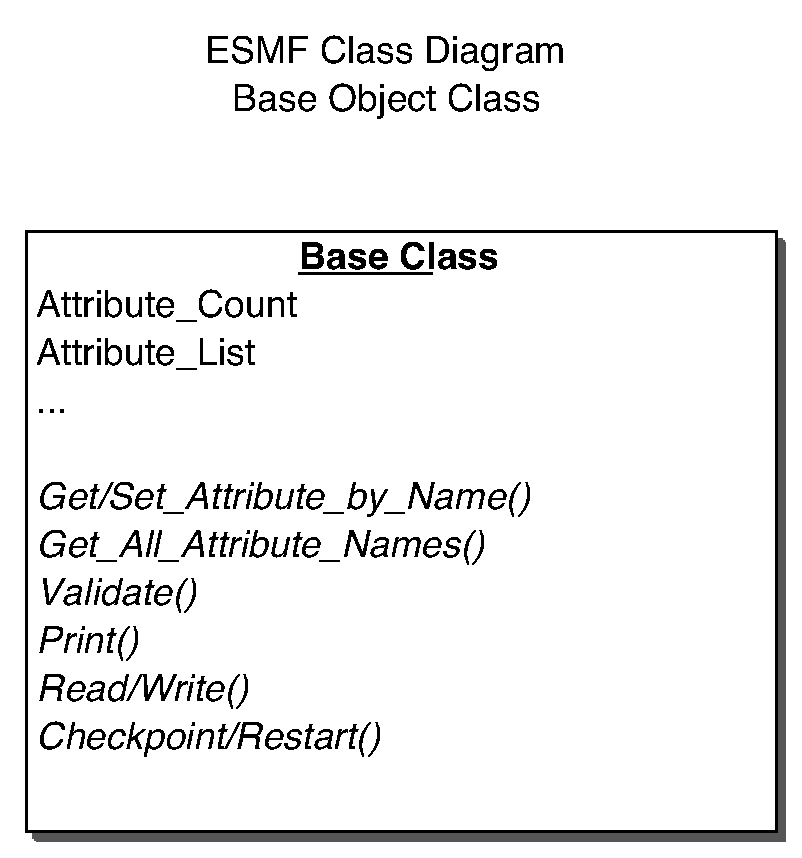
\includegraphics{ESMF_Base.eps}}

\subsubsection{Base (ESMF\_Base)}
\label{sec:Base} 
\begin{description}
\item [Description] The ESMF Base class is an abstraction of the private data and
methods common to all other object in the system.  Some methods and data can be
inherited direcly from the Base class; others are expected to be overloaded by
higher level objects.
\item [Function] The Base class methods which are expected to be overloaded by
more specialized objects include: Print, Validate, Read/Write, Checkpoint/Restart.
Methods which are inherited by all other classes include those which 
set and query object Attributes.
\end{description}

<< perhaps the usage section goes here, or perhaps this doesn't
belong here and does belong combined with the usage section >>









\section{Review Status}

\noindent{\bf Architecture Review} \\

\begin{tabular}{r p{1.3in} p{2in}}
{\bf Review Date:} & <Date> \\ \\
{\bf Reviewers:}   & <Reviewer>          & <Institution> \\
                   & <Reviewer>          & <Institution> \\
                   & <Reviewer>          & <Institution>
\end{tabular}

%\section{Glossary}
%\input{ESMF_glos}

%\section{Bibliography}
%\bibliography{comp} 
%\bibliographystyle{plain}
%\addcontentsline{toc}{section}{Bibliography}

\end{document}







